\chapter{Design and Implementation}
\label{chap:implementation}
In this chapter the developed regular Broker solution is presented. The tools used in the development phase, the interfaces by which the system interacts with the clients, and an UML representation of the Use Cases, for a better understanding of the system workflow, are presented.

\section{Design and Implementation of the Context Broker}
\label{sec:broker}
This work first implements a regular Context Broker, with no fault tolerance resources. Then, it proposes a strategy to give the Broker High Availability function.
 
\subsection{Platform Choice}
The programming language chosen for the development of this work was Python. 

The system was implemented over a stateless HTTP REST (Representational State Transfer) Interface. \cite{jakl2005representational}. For the RESTful implementation, Python Flask framework was used \cite{flask}. For the created web interfaces, Bootstrap was used  \cite{bootstrap} .

For data persistence, MongoDB was used.

\subsubsection{Python, PyCharm and GitHub}
\textbf{Python} is a powerful and easy to learn modern programming language \cite{python}. It was chosen because it represents a challenge, and to show that the system is independent of the programmed language, i.e., different applications can interact with each other in the architecture, regardless the programming language they were developed on; what matters is the content of the messages exchanged. The \textbf{PyCharm} Python IDE was used as the development environment \cite{pycharm}, along with \textbf{GitHub} for version control \cite{github}.

\subsubsection{Flask}
Flask is a web application framework for Python. It is very light and easy to use. It provides RESTful request dispatching, as it is used in this work. \cite{flask}

\subsubsection{MongoDB}
MongoDB is a document-oriented database, classified as NoSQL. It uses a key-document data storage model, where a document can be a complex data structure. Documents can contain many different key-value pairs, or even nested documents. MongoDB is a free and open-source software \cite{mongodb}.


\subsection{System Architecture}
In Figure \ref{fig:diagram} an overall diagram of the system is illustrated. Each node is a component of the system, and the arrows represent the interactions between them.

\begin{figure}[h]
	\centering
	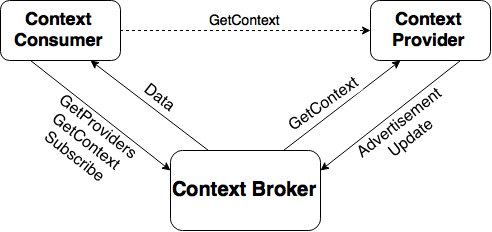
\includegraphics[scale=0.5]{diagram.png}
	\caption{Architecture diagram}
	\label{fig:diagram}
	
\end{figure}

\subsection{Data Collections}

As this work uses MongoDB to store data, the representation of Collections is used. Each Collection stores data in pair-value structure. As seen on Figure \ref{fig:collectionsdiagram}, the associations are made storing an entire object from a Collection inside another; this is made so it is easier to collect details about an associated element from another one.

\begin{figure}[h]
	\centering
	\includegraphics[scale=0.5]{collectionsdiagram.png}
	\caption{Collections diagram}
	\label{fig:collectionsdiagram}
	
\end{figure}



\subsection{Broker Interfaces}
The Context Broker implements several interfaces for communication with the other system components. This section presents each interface and the way they were implemented: what they expect as input (HTTP request from Consumer or Provider), the action they perform, and what they provide as output (response to the Consumer or Provider).


\subsubsection{Advertisement}
\begin{itemize}
	\item[Input:] an Advertisement ContextML message, with Provider information
	
	\item[Action:] registers the Provider within the Broker
	
	\item[Output:] responds the Provider with a ACK or NACK ContextML message, informing success or error, with the corresponding error message.
\end{itemize}

\subsubsection{Update (/update)}
\begin{itemize}
	\item[Input:] a ctxEl ContextML Message, with context information to be registered in the Broker
	
	\item[Action:] registers in the Registry Table the context information, with its \textit{contextProvider}, \textit{scope} and \textit{entity} information, \textit{timestamp} and expiration date (\textit{expires}) of the information. It also checks if a \textbf{Subscription} exists for the updated information, sending it to the Consumer \textit{callbackUrl}, when applied.
	
	\item[Output:] responds the Provider with a ACK or NACK ContextML message, informing success or error, with the corresponding error message.
\end{itemize}

\subsubsection{Get Providers (/getProviders)}
\begin{itemize}
	\item[Input:] \textit{scope} (mandatory) and \textit{entity type} (optional) arguments in the URL
	
	\item[Action:] looks for registered Providers that provide information matching the arguments given
	
	\item[Output:] responds the Consumer with Providers Lookup ContextML message, containing a list of the providers that match the requested arguments
\end{itemize}

\subsubsection{Get Context (/getContext)}
\begin{itemize}
	\item[Input:] from the Consumer, arguments \textit{scope} and \textit{entity} in the URL
	
	\item[Action:] looks for the latest Context information in the registry that matches the entity and scope received
	
	\item[Output:] responds the Consumer with a ctxEls ContextML message, containing the , or with a NACK ContextML message, informing the error.
	
\end{itemize}
* As seen in Figure \ref{fig:diagram}, there can also exist a direct \textit{GetContext} request from the Consumer to the Provider, thus not involving the Broker. This can be done by the Consumer asking the Broker for a providers list regarding a certain \textit{scope}, and then asking it directly for the desired context information. 

\subsubsection{Subscribe (/subscribe)}
\begin{itemize}
	\item[Input:] arguments as follows \textit{callbackUrl}, with the URL to where the Broker sends the content it is subscribed to; \textit{scope} and \textit{entity}, with corresponding information the consumer wants to subscribe to; and \textit{minutes}, with the amount of time, in minutes, that the subscription is valid.
	
	\item[Action:] registers the subscription
	
	\item[Output:] responds the Provider with a ACK or NACK ContextML message, informing success or error, with the corresponding error message.
\end{itemize}

\section{UML representation}
The interactions between the clients (Consumers and Providers) and the server (Broker) will be presented using the Unified Modeling Language, UML \cite{uml}.

\subsection{Use Case Requirements}
To present the Use Cases, a list of requirements is provided below. These requirements are adapted from a previous work \cite{crippa2010}, to the functions of this work.

\begin{enumerate}
	\item Register of Context Providers 
	\begin{description}
		\item (a) Receive Advertisement message 
		\item (b) Register CxP on Providers Table
	\end{description}
	\item Context Providers Lookup
	\begin{description}
		\item (a) Receive Providers Lookup request (GetProviders)
		\item (b) Answer with requested Providers data
	\end{description}
	\item Subscribe Context Consumer to data
	\begin{description}
		\item (a) Receive Subscription request
		\item (b) Register Subscription on Subscriptions table
	\end{description}
	\item Context data interactions
	\begin{description}
		\item (a) Receive Context data from a Context Provider (Update)
		\item (b) Send Context data to subscribed Consumers
		\item (c) Receive Context data request from a Context Consumer (GetContext) and respond
	\end{description}
\end{enumerate}

Both \textbf{Lookup} and \textbf{Register of Context Providers} services make the Broker aware of the existence of Context Providers in the network.

The rest of the requirements deal with context data provision and querying, by Providers and Consumers. The Providers see the Broker as the component where they send their context information, so Consumers can find and interpret it. The Consumers see the Broker as the centralized point from where to get up-to-date context data.


\subsection{Use Cases}
When a request from outside the system is received, the behavior is described in a \textbf{Use Case} \cite{bittner2002use}. In this work, the actors are the Context Broker, the Context Provider and the Context Consumer. The following list presents the use cases in the system. For the sake of brevity, the word Context will be omitted when referring to the actors.

\subsubsection{Registration of Providers}
\begin{itemize}
	\item[\textbf{Name}:] Register Provider
	\item[Actor(s):] Provider, Broker
	\item[Objective:] Register Provider from an Advertisement ContextML message received from it
	\item[Description:] Validates the ContextML message against the ContextML schema, then registers the Provider and its capabilities (e.g. scopes and entity types it covers) in the Broker 
	\item[Type:] Primary and Essential
	\item[References:] Requirements 1.a, 1.b 
	\item[Sequence of Events:]\hfill
		\begin{enumerate}
			\item Provider sends a POST HTTP message containing an Advertisement ContextML message to the \textit{/advertisement} interface of the Broker
			\item The Broker receives and validates the message
				\begin{itemize}
					\item If not valid, the Broker sends a NACK ContextML message to the Provider
					\item If valid, the Broker registers the Provider if new, or updates its information if already existent. If there is an error during the process, a NACK ContextML message is sent to the Provider.
				\end{itemize}
			\item The Broker sends an ACK ContextML message to the Provider, the registration was successful
		\end{enumerate}
\end{itemize}

\subsubsection{Provider Lookup service}
\begin{itemize}
	\item[\textbf{Name}:] Receive Provider Lookup request
	\item[Actor(s):] Consumer, Broker
	\item[Objective:] Receive, validate and find Providers that match the arguments received from the Consumer
	\item[Description:] The Broker is the only component of the system that has information about all the Providers, thus if a Consumer wants to know where to find a specific information (matching a particular scope or entity), it must ask the Broker for a list of Providers that provide this information.
	\item[Type:] Primary and Essential
	\item[References:] Requirement 2.a 
	\item[Sequence of Events:]\hfill
	\begin{enumerate}
		\item Consumer sends a GET HTTP message to the Broker's \textit{/getProviders} interface, with \textit{scope} and \textit{entity type} arguments in the URL.
		\item The Broker validates the arguments: the scope argument is mandatory, while the entity is optional
		\begin{itemize}
			\item If the scope argument is blank, the Brokers responds to the Consumer with a NACK ContextML message, informing the \textit{Bad Parameter} error, in the error message
			\item If the scope is valid, the Broker searches at its internal information for the Providers that match the requested scope and entity type
		\end{itemize}
		\item The Respond Provider Lookup request is started
	\end{enumerate}
\end{itemize}

\begin{itemize}
	\item[\textbf{Name}:] Respond Provider Lookup request
	\item[Actor(s):] Consumer, Broker
	\item[Objective:] Respond to the Consumer a list of Context Providers that match the information requested (\textit{scope}and \textit{entity type})
	\item[Description:] The Broker creates a Providers Lookup ContextML message with the information of the Providers that match the search criteria, and sends it to the Consumer
	\item[Type:] Primary and Essential
	\item[References:] Requirement 2.b 
	\item[Sequence of Events:]\hfill
	\begin{enumerate}
		\item The Broker creates the Providers Lookup ContextML message with the desired Providers. If no Providers match the search criteria, a NACK ContextML message is created, informing \textit{No results found} in the error message
		\item The resulting message is sent to the Consumer
	\end{enumerate}
\end{itemize}

\subsubsection{Subscribe Consumer to data}
\begin{itemize}
	\item[\textbf{Name}:] Register Subscription from Consumer
	\item[Actor(s):] Consumer, Broker
	\item[Objective:] Register a Subscription made by a Consumer, to a certain \textit{entity id}, \textit{entity type} and \textit{scope} combination
	\item[Description:] The Subscription system provided by the Broker is a way of a Consumer to receive any new context information as soon as it is received by the Broker, within a given entity and scope combination. The Subscription is valid for a certain amount of time, defined by the Consumer. The Consumer also informs the Broker a callback URL, to where the Broker sends the new context information the Consumer is subscribed to.
	\item[Type:] Primary and Essential
	\item[References:] Requirements 3.a, 3.b 
	\item[Sequence of Events:]\hfill
	\begin{enumerate}
		\item The Consumer sends a POST HTTP message to the \textit{/subscribe} interface of the Broker, with \textit{entity}, \textit{scopeList}, \textit{callbackUrl} and \textit{minutes} arguments in the URL
		\item The arguments are validated, 
		\begin{itemize}
			\item If any is blank or the minutes value is less than one (1), a NACK ContextML message is sent to the Consumer
			\item If all arguments are valid, the Broker checks if the information given in the arguments exists within the Broker. If not, a NACK ContextML message is sent to the Consumer
		\end{itemize}
		\item The Subscription is registered in the Subscriptions table in the Broker
		\item A timer is started for the subscription
		\item An ACK ContextML message is sent to the Consumer, the Subscription was successful
	\end{enumerate}
\end{itemize}

\begin{itemize}
	\item[\textbf{Name}:] Check if Subscription expired
	\item[Actor(s):] Broker
	\item[Objective:] Check if timer to a Subscription runs out
	\item[Description:] When the Subscription is registered, it has a \textit{minutes} argument that states for how long this Subscription is valid. When this time runs out, the Subscription is removed.
	\item[Type:] Primary and Essential
	\item[References:] Requirement 3.b 
	\item[Sequence of Events:]\hfill
	\begin{enumerate}
		\item The timer related to a Subscription runs out
		\item The Broker initiates the removal of the Subscription
		\item The Subscription is removed from the Subscriptions table
	\end{enumerate}
\end{itemize}

\subsubsection{Context data interactions}
\begin{itemize}
	\item[\textbf{Name}:] Receive Update message from Provider
	\item[Actor(s):] Provider, Broker
	\item[Objective:] Receive and store context data sent from a Provider
	\item[Description:] New context data is sent from the Provider to the Broker. The Broker must store it, and check if there's any Subscription related to the data stored, sending the data if a Subscription exists.
	\item[Type:] Primary and Essential
	\item[References:] Requirement 4.a
	\item[Sequence of Events:]\hfill
	\begin{enumerate}
		\item Provider sends a POST HTTP message to the \textit{/update} interface of the Broker, containing a Context Element ContextML message with the context data information
		\item The Broker validates the message agains the ContextML schema
			\begin{itemize}
				\item If the message fails the validation, a NACK ContextML message is sent to the Provider
				\item If it validates, the Broker checks if the Provider is registered and if the scope receiving data is valid. 
				\begin{itemize}
					\item If the Provider is not registered or the scope is invalid, the Broker sends a NACK ContextML message to the Provider
					\item If the information is valid, the Broker sees if the entity id and entity type already exist; if not, they are created
				\end{itemize}
			\end{itemize}
			
			\item The data is registered in the Broker, with its timestamp and expiration time. If there had already information about this entity and scope, that is considered deprecated and this is the newest data
			\item The Send context data to subscribed Consumer use case is initiated
	\end{enumerate}
\end{itemize}

\begin{itemize}
	\item[\textbf{Name}:] Send context data to subscribed Consumer
	\item[Actor(s):] Broker, Consumer
	\item[Objective:] Check if any Subscription is related to the just updated context data, and send this data to a Consumer that is subscribed
	\item[Description:] After registering the new context data, the Broker looks at the Subscriptions table for a Subscription related to the entity id, entity type and scope of the new data. If it exists, the Broker sends the same Context Element ContextML message to the Consumer in the Subscription.
	\item[Type:] Primary and Essential
	\item[References:] Requirement 4.b
	\item[Sequence of Events:]\hfill
	\begin{enumerate}
		\item The Broker checks the Subscriptions table, trying to match the entity id, entity type and scope of the context data just registered
		\item If no Subscription is found, the Broker sends an ACK ContextML message to the Provider after the update
		\item If a Subscription is found, the Broker sends the same Context Element ContextML message it received from the Provider to the subscribed Consumer
		\item Then the Broker sends an ACK ContextML message to the Provider after the update
	\end{enumerate}
\end{itemize}


\begin{itemize}
	\item[\textbf{Name}:] Receive context request from Consumer
	\item[Actor(s):] Consumer, Broker
	\item[Objective:] Receive a request for context data
	\item[Description:] A Consumer can ask specific context data to the Broker, defining a list of scopes and an entity it wants the last information about
	\item[Type:] Primary and Essential
	\item[References:] Requirement 4.c
	\item[Sequence of Events:]\hfill
	\begin{enumerate}
		\item The Consumer sends a GET HTTP message to the \textit{/getContext} interface of the Broker, with \textit{scopeList} and \textit{entity} arguments in the URL
		\item The Broker validates the arguments, checking if the entity and scopes requested exist in the registered data
		\item If the arguments are valid, the Broker sends an ACK ContextML message to the Consumer
		\item If not, the Broker makes an extra effort, as the Request Provider for context data not found in the Broker use case begins
	\end{enumerate}
\end{itemize}

\begin{itemize}
	\item[\textbf{Name}:] Request Provider for context data not found in the Broker
	\item[Actor(s):] Provider, Broker
	\item[Objective:]
	\item[Description:]
	\item[Type:] Primary and Essential
	\item[References:] Requirement 4.c
	\item[Sequence of Events:]\hfill
	\begin{enumerate}
		\item The Broker sends to the Provider the same context data request it received from the Consumer
		\item If the Provider responds with context data, the Broker sends it to the Consumer
		\item If the Provider responds with no data found, the Broker sends a NACK ContextML message to the Consumer, informing that no data was found
	\end{enumerate}
\end{itemize}

\subsection{Use Cases Diagrams}
A Use Case Diagram present a good view of the actors and actions of the system.
For the sake of clarity, in Figure \ref{fig:usecases} an overview of the use cases is presented. More detailed diagrams of the modules can be seen on Figure \ref{fig:register}, Figure \ref{fig:lookup}, Figure \ref{fig:subscribe} and Figure \ref{fig:contextdata}


\begin{figure}[h]
	\centering
	\includegraphics[scale=0.5]{usecases.png}
	\caption{Overview of the Use Cases}
	\label{fig:usecases}
	
\end{figure}


\begin{figure}[h]
	\centering
	\includegraphics[scale=0.5]{register.png}
	\caption{Register Provider Use Case detail}
	\label{fig:register}
	
\end{figure}


\begin{figure}[h]
	\centering
	\includegraphics[scale=0.5]{lookup.png}
	\caption{Provider Lookup Use Case detail}
	\label{fig:lookup}
	
\end{figure}


\begin{figure}[h]
	\centering
	\includegraphics[scale=0.5]{subscribe.png}
	\caption{Subscribe Use Case detail}
	\label{fig:subscribe}
	
\end{figure}


\begin{figure}[h]
	\centering
	\includegraphics[scale=0.5]{contextdata.png}
	\caption{Context data interactions Use Case detail}
	\label{fig:contextdata}
	
\end{figure}

\section{Proposition of High Availability Technique}
\label{sec:ha_broker}
The objective here is to design a system of Brokers that present high availability behavior. The idea proposed here is inspired by concepts explained on \ref{sec:fault_tolerance}, aiming at a cluster-like behavior from the Broker system. For the sake of brevity, both Provider and Consumer will be referred to as \textit{client}.

\subsection{Requirements}
As availability is measured from the user's point of view, some basic requirements for a highly available Context Broker are described below:

\begin{itemize}
	\item Clients should always be able to query data from the Broker
	\item Clients should always be able to insert data to the Broker
	\item Context data should always be consistent, i.e., different interfaces should provide the exact same information at the same time
	\item Every request made by a client should be answered, either by the same Broker it sent the request or by another one in the case of a failure of the first
\end{itemize}

\subsection{Design}
Following the requirements on the previous section, the idea is to use a Symetric Active/Active redundancy technique, having multiple redundant active components, with the data collection state actively replicated among them, using commit protocols. Data collection state is shared in form of a global state. This provides continuous availability without any interruption and without wasting resources \cite{engelmann2005concepts}.

The Broker System, illustrated at Figure \ref{fig:brokersystem}, is composed of a predefined number of Brokers, each one with its own IP address, running independently from the others, connected on a local network. They can be accessed at the same time from different clients. The clients should have a list of the IPs from the Broker system. Each Broker may have an interface to which a client can query the addresses of the other Brokers in the same system, but the clients must know at least one of the Brokers, there is no discovery method. If a Broker fails not during a request, a client won't be able to reach it, and then will try the next Broker address of the system.


\begin{figure}[h]
	\centering
	\includegraphics[scale=0.5]{brokersystem.png}
	\caption{Broker System for High Availability}
	\label{fig:brokersystem}
	
\end{figure}



All the Brokers present the same data collection, with strong consistency \cite{vogels2009eventually}. 


\subsection{Proposed Protocol}

There are two types of operations a request from a client can inflict in the data collection of the Broker system: \textbf{select} and \textbf{insert}.

When the operation is a \textbf{select}, there's no need to worry about the consistency of the data collection, as no changes are made to it. However, on an \textbf{insert}, the Broker system must guarantee the consistency of the global data collection state. This is done through a three-phase commit protocol inspired by \cite{guerraoui2002non}.


In the first phase (\textbf{prepare}), the Broker that received the requests sends a broadcast message with the request, and waits until everyone has sent an ACK message to another. The second phase (\textbf{pre-commit}) is where all the Brokers communicate to each other that they are ready to commit, i.e., ready to insert the new value in the data collection. All the Brokers wait for the ACK messages from every one. The third phase (\textbf{commit}) is where all the Brokers make the insertion in the data collection, and finally after the Broker that received the request responds its client, it broadcasts a message informing everyone that the request was completed. If a single ACK message is not received in any part of the cycle, it means one of the Brokers is down. If it is the Broker that received the request, one of the remaining ones should respond the client. The decision of which Broker responds the client falls under an election problem, a simple solution would be giving a order of priority for replacement scenarios, but the study of a more complex solution is suggested as future work. This ensures that the client is answered even if the Broker to whom the request was made goes down. The operation is not aborted, unless all the Brokers are down.


For the \textbf{select} operations, a similar idea is used, differing only in the case that there are only two phases: prepare and select. The \textbf{prepare} phase is the same as with the insert operations, all the Brokers communicate that they all have received a copy of the request; when they all confirm that received it using ACK messages, the second phase (\textbf{select}) begins. All the Brokers make the select operation on its own data collection. The Broker that received the request then responds the client and broadcasts to all the others a message informing that the request was a success, while these others don't respond the client, but wait for the confirmation that the first one did it. If any of these confirmation messages fail, the remaining Brokers will notice which Broker failed and, if it was the one that received the original request, one of the remaining Brokers responds the client, using the data it had already selected from the data collection.

In Figure \ref{fig:protocoldiagram} the behavior of a Broker given a particular request is illustrated using a state diagram. The following notation is used: \textit{ro$_i$} stands for the request-original's initial state, i.e. the Broker that received the request, and \textit{b$_i$} represents the initial state of the remaining Brokers. They may have different initial states, but they act the same way from the second state on. \textit{p}, \textit{pc} and \textit{c} stand for the \textbf{prepare}, \textbf{pre-commit} and \textbf{commit} phases, respectively. The \textit{commit} action can be interpreted as either \textbf{insert} or \textbf{select} atomic operation on each Broker's data collection.

\begin{figure}
	\centering
	\includegraphics[scale=0.4]{protocoldiagram.png}
	\caption{State Diagram for proposed protocol}
	\label{fig:protocoldiagram}
	
\end{figure}


The time-out value of the messages between the Brokers is an important decision: a large value is better for avoiding false-suspicions, while a small one is better for a quicker response to failures; one can use even a dynamic time-out value, that grows until it reaches a decision \cite{guerraoui2002non}. It is up to the system designer to define an optimal time-out value.

This proposed protocols is to be used for single-failure scenarios. A solution for a bigger amount of failures depends on solving the election problem when one Broker fails. Also, given the failure of a Broker, it must pass through a recovering state when restarted. A recovering mechanism for the highly available Broker system is suggested as future work.


A common problem in this kind of approach is the insertion order when two clients try to insert values regarding the same data at the same time, not leaving enough time for the message exchanges to complete. However, it is not possible in this system due to the way Context is structured. The order of insertion is defined by the client. It is not possible that two clients try to insert values regarding the same Context data at the same time, as each Context Provider provides its own data, which does not interfere with other Providers data. The same applies to Consumers.